\chapter{QuB Express}

There are two main versions:
\begin{enumerate}
  \item QUB Classic: simulates, or acquires + pre-process + analyze ion channels
  data measured instruments
  \item QUB Express: interactively simulate ion channel and analyse it.
\end{enumerate}

In this chapter, we learn how to build a model using QuB Express.
\url{http://www.qub.buffalo.edu/wiki/index.php/Video_Lessons}

\url{http://www.qub.buffalo.edu/wiki/index.php/Main_Page}

QuB express has 6 main panels: Model, Tables, Scope, Tools, Details, and
Text-out.\footnote{\url{http://www.qub.buffalo.edu/wiki/index.php/QUB_Express}}.

\section{Models, Tables}
\label{sec:model_tables}

The two main components (Models, Tables) in the GUI of QuB Express is showed in
Fig.\ref{fig:QuB_Express_01}. The second part allows us to modify the Markov
model by adding/removing states, and adjust the connectivity between states.
By default, you will have a two-state Markov model. The first part has different
tables that allow us to modify different aspects of the given model.

\begin{figure}[hbt]
  \centerline{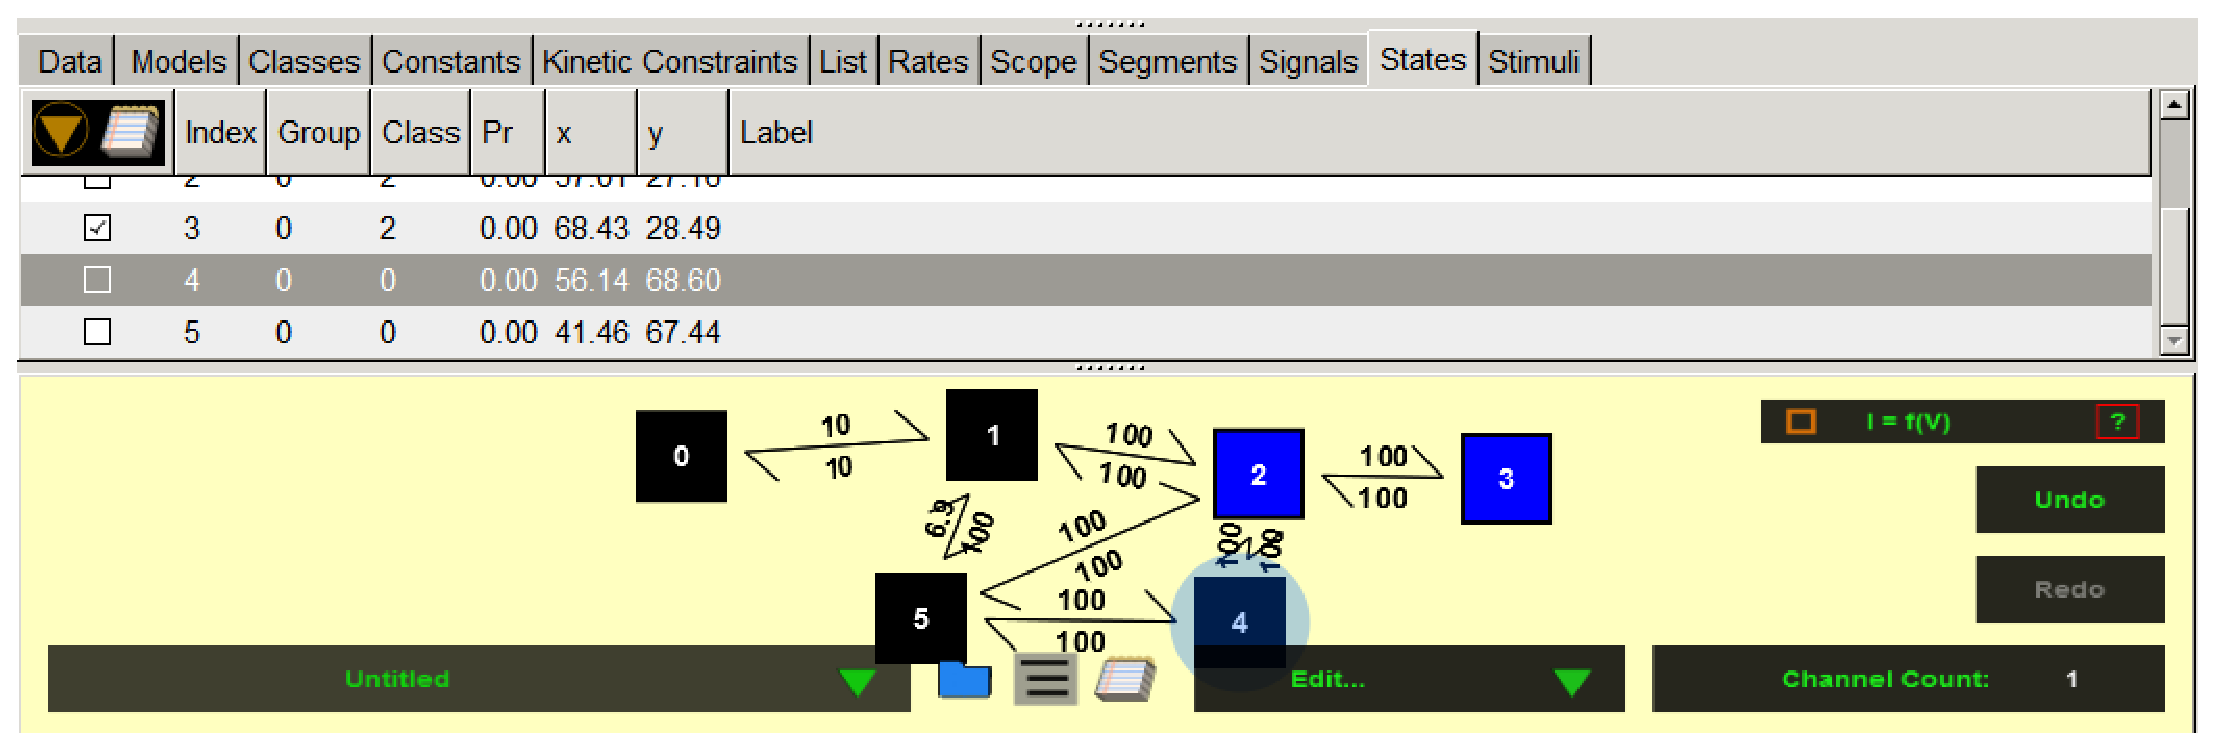
\includegraphics[height=5cm,
    angle=0]{./images/QuB_Express_01.eps}}
  \caption{Two components in the GUI of QuB Express}
  \label{fig:QuB_Express_01}
\end{figure}

A model is like a graph, with {\it states} as vertex, and {\it transition rates}
as connecting edges. A new state can be added by clicking on the second part and
choose ``New State''. There, you need to choose a color for that new state. The
color represents a {\it class} of states that have the same conducting level.
Typically, {\bf black} means no conducting. The definition of the conducting
level for each class of states is given in the {\bf CLASS table} in the first
component, Fig.\ref{fig:QuB_Express_02}. Apart from grouping channels of the
same conducting level, we have a secondary mechanism to group states using Group
index. There, we have:
\begin{enumerate}
  \item Index: the index of the class (managed by the system)
  \item Group: a secondary mechanism to group states
  \item Amp:  the mean current amplitude (unit = pA) (0=no conducting,
  1=conducting at 1pA, 2=conducting at 2pA)
  \item Std: standard deviation of the Gaussian noise about the mean {\bf Amp}
  (unit = pA)
  \item Cond: the mean conductance (unit = pS) in pico Siemens
  \item CondStd: standard deviation of the Cond
  \item vRev: is the reversal potential $E_\rev$ (unit: Volt)
\end{enumerate}
Depending on how you choose to model the current, it can either use (Amp, Std)
or (Cond, CondStd). If we use (Cond, CondStd), then the current is calculated
based on
\begin{verbatim}
pA = pS * (V - vRev)
\end{verbatim}
NOTE: The voltage must be in (Volt).


\begin{figure}[hbt]
  \centerline{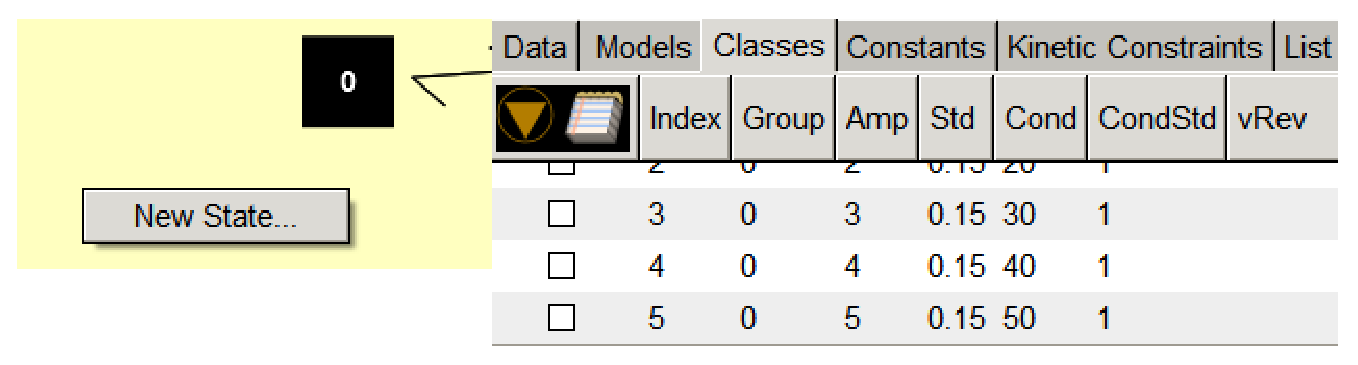
\includegraphics[height=3cm,
    angle=0]{./images/QuB_Express_02.eps}}
  \caption{(A) Add new state, (B) Adjust {\bf class} for each state}
  \label{fig:QuB_Express_02}
\end{figure}


Now, jump to the {\bf STATE table} where we can modify individual states'
properties. 
\begin{enumerate}
  \item Index: the index of the class (managed by the system)
  \item Group: a secondary mechanism to group states
  \item Class:
  \item Pr: initial probability for the channels in that state (NOT BEING USED
  if we choose {\it Start at Equilibrium} (Fig.\ref{fig:QuB_Express_03}))
  \item x, y: the coordinates of the state on the Model panel 
  \item Label: Label for the states in graph
\end{enumerate}

Now, jump to the {\bf RATES table} where we modify the transition rates which is
defined using the general formula
\begin{verbatim}
k = k0 * Ligand * e^(k1 * Voltage)
\end{verbatim}
with 
\begin{enumerate}
  \item \verb!Ligand! is where you define how the transition is a function of
ligand concentration, e.g. if the rate follows $([\Ca]_\ds)^2$ then we write 
\verb!Cads^2! with \verb!Cads! is a variable that we need to define then.
  \item \verb!Voltage! is where you define how the transition is a function of
  voltage, e.g. if the rate follow \verb!-(V-10)/20!, then we write
  \verb!(Vm-10)! with \verb!k1=-1/20! and \verb!Vm! is the membrane potential
  that we need to define then.
\end{enumerate}
The two important coefficients are \verb!k0! pre-exponential coefficient and
\verb!k1! exponential coefficient.

If your model has a loop, then you can add kinetic constraint to the model using
{\bf KINETIC CONSTRAINT table}. 
\begin{enumerate}
  \item Balance all loops: for microscopic reversibility. Selects the states in
  the loop by modifying States column in the table

Example: 
  \item Add row: 
  \item Delete row: delete an existing constraint
\end{enumerate}

If we want the rate to become more likely with positive $V_m$ then make
\verb!k1! positive; otherwise makes it negative.

\section{Scopes}

After you have created the model (Sect.\ref{sec:model_tables}), the output of
the simulation is showed in component {\bf Scopes} which looks like the
oscilloscope. To modify how you want the simulation to be, select and
modify: Sampling frequency, Start at Equilibrium, etc.
Fig.\ref{fig:QuB_Express_03}.


\begin{figure}[hbt]
  \centerline{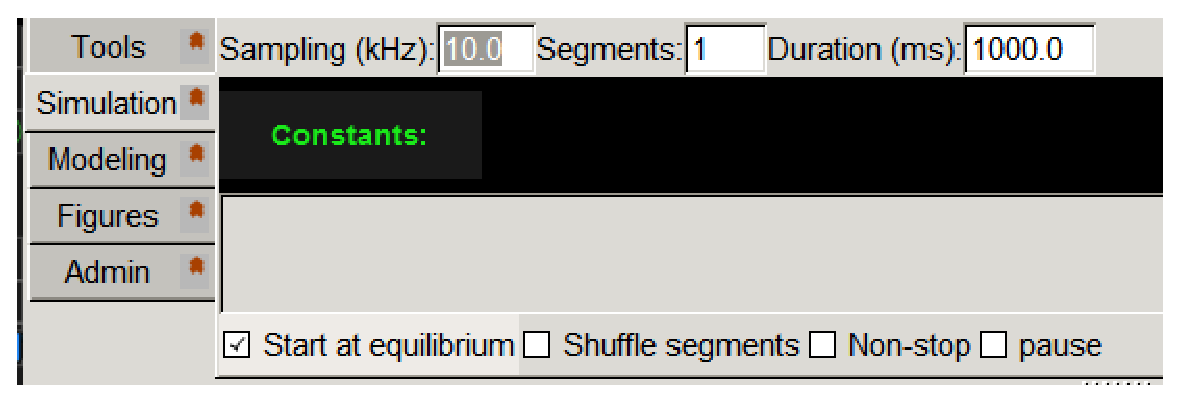
\includegraphics[height=3cm,
    angle=0]{./images/QuB_Express_03.eps}}
  \caption{How you want the simulation to be}
  \label{fig:QuB_Express_03}
\end{figure}


The data consists of one or more parallel signals. The first signal (index=0) is
the Markov model to be analyzed. Other signals can be data from other variables,
e.g. ligand concentration, transmembrane voltage, etc.

A signal is a list of segments (default = 1). We can add more segments by
changing Segments, Fig.\ref{fig:QuB_Express_03}. The duration of the simulation
for each Segment is given next to that textbox. The output frequency for each
Segment is given in the left textbox. As we can see in the Scope panel, the
Segment contains ``events'' (aka ``dwells''), or a class of amplitude values.
Essentially, for each signal we have
\begin{verbatim}
[(classes[], durations[], amp_of_cls[]), ...]
\end{verbatim}

\url{http://www.qub.buffalo.edu/src/qub-express/api/qubx_single_molecule/max_subi_ll.py}

\section{Simulate}

After we have setup the model (Sect.\ref{sec:model_tables}), we can now run the
Simulation with either (1) at Equilibrium, (2) responding to a stimulus
protocol.

\section{Parameter Estimations}

If you already have the model, i.e. with proper connections, and you want to
estimate the parameter, then this is the right section.


\section{Model Search}

After we have setup the model (Sect.\ref{sec:model_tables}), we can now use
Modeling\\Util tab, Fig.\ref{fig:QuB_Express_04}. Select ModelSearch from
Utilities and proper Optimizer
\begin{enumerate}
  \item MacroR
  \item MacRates
  \item MIL (Maximum Interval
  Likelihood):\url{http://www.qub.buffalo.edu/wiki/index.php/Modeling:MIL}
  \item MSL
  
\end{enumerate}

\url{http://www.qub.buffalo.edu/wiki/index.php/Modeling:Model_Search}

\begin{figure}[hbt]
  \centerline{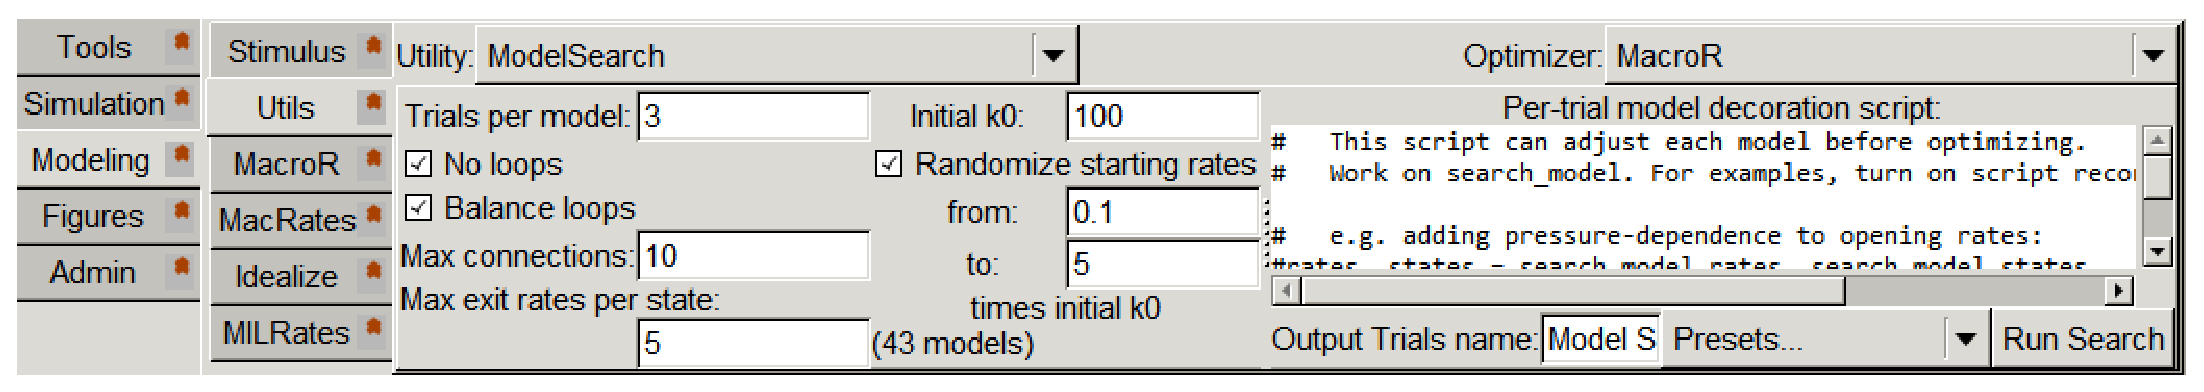
\includegraphics[height=2cm,
    angle=0]{./images/QuB_Express_04.eps}}
  \caption{Model search}
  \label{fig:QuB_Express_04}
\end{figure}

Other options:
\begin{enumerate}
  \item No loops: skip connection scheme with cycles of 3 or more states
  \item Balance loops: constrain all cycles to be in a detailed balance. Tricks:
  \url{http://www.qub.buffalo.edu/wiki/index.php/How_to_satisfy_cycle_(im)balance}
  \item Max connections: skip connection scheme with too many total connections 
  \item Max exit rates per state: skip connection scheme with too many connections from a
  single state
  \item Initial k0: starting value for all pre-exponential terms. If we don't
  want them to have the same starting value, we can multiply each of them
  with a number randomly chosen in the range specified by \verb!Randomize!
  \verb!starting rates!
  \item Randomize starting rates: 
  
\end{enumerate}



\section{QUB Express code}

We need g++, boost, python, pygtk, gtk++2, pycairo, argparse, numpy and scipy.
QUB Express was released in 2010. 
